\documentclass[12pt,a4paper]{article}

% ============================================
% PAQUETES
% ============================================
\usepackage[utf8]{inputenc}
\usepackage[spanish]{babel}
\usepackage{amsmath,amssymb,amsthm}
\usepackage{graphicx}
\usepackage{float}
\usepackage{booktabs}
\usepackage{array}
\usepackage{longtable}
\usepackage{hyperref}
\usepackage{xcolor}
\usepackage{listings}
\usepackage{geometry}
\usepackage{fancyhdr}
\usepackage{titlesec}
\usepackage{caption}
\usepackage{subcaption}
\usepackage{tikz}
\usetikzlibrary{automata,positioning,arrows}

% ============================================
% CONFIGURACIÓN
% ============================================
\geometry{margin=2.5cm}
\hypersetup{
    colorlinks=true,
    linkcolor=blue!70!black,
    urlcolor=blue!70!black,
    citecolor=green!50!black
}

% Configuración de listings para código
\lstset{
    basicstyle=\ttfamily\small,
    backgroundcolor=\color{gray!10},
    frame=single,
    breaklines=true,
    numbers=left,
    numberstyle=\tiny\color{gray},
    keywordstyle=\color{blue},
    commentstyle=\color{green!60!black},
    stringstyle=\color{red!70!black},
    showstringspaces=false
}

% Headers y footers
\pagestyle{fancy}
\fancyhf{}
\fancyhead[L]{\small Máquina de Turing - Fibonacci}
\fancyhead[R]{\small ADA 2026}
\fancyfoot[C]{\thepage}
\renewcommand{\headrulewidth}{0.4pt}

% Definiciones matemáticas
\newtheorem{definicion}{Definición}
\newtheorem{teorema}{Teorema}
\newtheorem{lema}{Lema}

% ============================================
% DOCUMENTO
% ============================================
\begin{document}

% ============================================
% PORTADA
% ============================================
\begin{titlepage}
    \centering
    \vspace*{1cm}
    
    {\Large\bfseries Universidad del Valle de Guatemala\par}
    \vspace{0.5cm}
    {\large Facultad de Ingeniería\par}
    {\large Ingeniería en Ciencias de la Computación y Tecnologías de la Información\par}
    
    \vspace{2cm}
    
    \rule{\textwidth}{1.5pt}\par
    \vspace{0.5cm}
    {\Huge\bfseries Máquina de Turing para la\\[0.3cm]Sucesión de Fibonacci\par}
    \vspace{0.5cm}
    \rule{\textwidth}{1.5pt}\par
    
    \vspace{1.5cm}
    
    {\Large\itshape Análisis de Complejidad Temporal\\con Notación Asintótica O\par}
    
    \vspace{2cm}
    
    {\large\bfseries Proyecto 1\par}
    \vspace{0.3cm}
    {\large Análisis y Diseño de Algoritmos\par}
    
    \vfill
    
    {\large 
        Javier Eduardo España Pacheco #23361\par
    }
    
    \vspace{1.5cm}
    
    {\large 27 de Febrero, 2026\par}
\end{titlepage}

% ============================================
% ÍNDICE
% ============================================
\tableofcontents
\newpage

% ============================================
% RESUMEN
% ============================================
\section*{Resumen}
\addcontentsline{toc}{section}{Resumen}

Este proyecto presenta el diseño, implementación y análisis de una \textbf{Máquina de Turing determinista de una cinta} que calcula el n-ésimo número de la sucesión de Fibonacci. Se utiliza representación unaria de números y un enfoque iterativo que mantiene los términos de la secuencia en la cinta.

El análisis teórico demuestra que la complejidad temporal es \textbf{exponencial}, específicamente $O(\varphi^{2n}) \approx O(2.618^n)$, donde $\varphi$ es la proporción áurea. Esta complejidad se verifica empíricamente mediante la medición del número de pasos y tiempo de ejecución para diferentes valores de $n$.

La máquina final cuenta con \textbf{24 estados} y \textbf{58 transiciones}, incluyendo una verificación de paridad inicial mediante estados alternantes. Los resultados experimentales confirman el crecimiento exponencial predicho, con un ratio de crecimiento $T(n)/T(n-1)$ que converge hacia $\approx 2.59$.

\textbf{Palabras clave:} Máquina de Turing, Fibonacci, Complejidad Temporal, Notación O, Crecimiento Exponencial.

\newpage

% ============================================
% 1. INTRODUCCIÓN
% ============================================
\section{Introducción}

\subsection{Contexto}

Las Máquinas de Turing, propuestas por Alan Turing en 1936, constituyen uno de los modelos computacionales más fundamentales en ciencias de la computación. A pesar de su simplicidad teórica, son capaces de computar cualquier función que sea efectivamente calculable (tesis de Church-Turing).

La sucesión de Fibonacci, definida por la recurrencia $F(n) = F(n-1) + F(n-2)$ con $F(0)=0$ y $F(1)=1$, es un problema clásico que permite estudiar diferentes complejidades algorítmicas según la implementación elegida.

\subsection{Objetivos}

\begin{enumerate}
    \item Diseñar una Máquina de Turing determinista de una cinta que calcule $F(n)$
    \item Implementar un simulador en Python para ejecutar y analizar la máquina
    \item Determinar la complejidad temporal usando notación asintótica O
    \item Verificar empíricamente el análisis teórico mediante mediciones experimentales
\end{enumerate}

\subsection{Alcance}

Este proyecto implementa una MT de una sola cinta con representación unaria, lo que resulta en una complejidad exponencial. No se optimiza para eficiencia práctica, sino para demostrar los conceptos fundamentales de análisis de algoritmos.

\newpage

% ============================================
% 2. MARCO TEÓRICO
% ============================================
\section{Marco Teórico}

\subsection{Máquinas de Turing}

\begin{definicion}[Máquina de Turing]
Una \textbf{Máquina de Turing determinista} es una 7-tupla $M = (Q, \Sigma, \Gamma, \delta, q_0, q_{accept}, q_{reject})$ donde:
\begin{itemize}
    \item $Q$ es el conjunto finito de estados
    \item $\Sigma$ es el alfabeto de entrada (no incluye el blanco)
    \item $\Gamma$ es el alfabeto de la cinta ($\Sigma \subseteq \Gamma$)
    \item $\delta: Q \times \Gamma \rightarrow Q \times \Gamma \times \{L, R, S\}$ es la función de transición
    \item $q_0 \in Q$ es el estado inicial
    \item $q_{accept} \in Q$ es el estado de aceptación
    \item $q_{reject} \in Q$ es el estado de rechazo
\end{itemize}
\end{definicion}

\subsection{Notación Asintótica O (Big-O)}

\begin{definicion}[Notación O]
Sean $f(n)$ y $g(n)$ funciones de los enteros no negativos a los reales. Decimos que:
$$f(n) = O(g(n))$$
si existen constantes positivas $c$ y $n_0$ tales que:
$$f(n) \leq c \cdot g(n) \quad \text{para todo } n \geq n_0$$
\end{definicion}

\subsubsection{Propiedades Importantes}

\begin{enumerate}
    \item \textbf{Transitividad:} Si $f(n) = O(g(n))$ y $g(n) = O(h(n))$, entonces $f(n) = O(h(n))$
    \item \textbf{Regla de la suma:} $O(f(n)) + O(g(n)) = O(\max(f(n), g(n)))$
    \item \textbf{Regla del producto:} $O(f(n)) \cdot O(g(n)) = O(f(n) \cdot g(n))$
\end{enumerate}

\subsection{Sucesión de Fibonacci}

La sucesión de Fibonacci se define recursivamente como:
\begin{align}
    F(0) &= 0 \\
    F(1) &= 1 \\
    F(n) &= F(n-1) + F(n-2) \quad \text{para } n \geq 2
\end{align}

Los primeros términos son: 0, 1, 1, 2, 3, 5, 8, 13, 21, 34, 55, 89, 144, ...

\subsubsection{Fórmula de Binet}

El n-ésimo número de Fibonacci puede expresarse mediante:
$$F(n) = \frac{\varphi^n - \psi^n}{\sqrt{5}}$$

Donde:
\begin{itemize}
    \item $\varphi = \frac{1 + \sqrt{5}}{2} \approx 1.618$ (proporción áurea)
    \item $\psi = \frac{1 - \sqrt{5}}{2} \approx -0.618$
\end{itemize}

Como $|\psi| < 1$, para $n$ grande: $F(n) \approx \frac{\varphi^n}{\sqrt{5}}$, por lo tanto $F(n) = \Theta(\varphi^n)$.

\newpage

% ============================================
% 3. DISEÑO DE LA MÁQUINA DE TURING
% ============================================
\section{Diseño de la Máquina de Turing}

\subsection{Especificación Formal}

La Máquina de Turing diseñada tiene las siguientes características:

\begin{itemize}
    \item \textbf{Tipo:} Determinista de una cinta
    \item \textbf{Estados:} 24
    \item \textbf{Transiciones:} 58
    \item \textbf{Alfabeto de entrada:} $\Sigma = \{1\}$
    \item \textbf{Alfabeto de cinta:} $\Gamma = \{1, \_, \#, ., ;, x, y, z\}$
\end{itemize}

\subsection{Convenciones de Representación}

\subsubsection{Notación Unaria}

Los números enteros no negativos se representan en \textbf{notación unaria}:

\begin{table}[H]
\centering
\begin{tabular}{cc}
\toprule
\textbf{Número} & \textbf{Representación} \\
\midrule
0 & (vacío) \\
1 & 1 \\
2 & 11 \\
3 & 111 \\
n & n unos \\
\bottomrule
\end{tabular}
\caption{Representación unaria de números}
\end{table}

\subsubsection{Alfabeto de la Cinta}

\begin{table}[H]
\centering
\begin{tabular}{cl}
\toprule
\textbf{Símbolo} & \textbf{Significado} \\
\midrule
\texttt{1} & Dígito unario (representa cantidad) \\
\texttt{\_} & Blanco (símbolo por defecto) \\
\texttt{\#} & Marcador de inicio de cinta \\
\texttt{.} & Separador zona de contador y trabajo \\
\texttt{;} & Separador entre términos Fibonacci \\
\texttt{x} & Contador usado/procesado \\
\texttt{y} & Marcador temporal copiando término 1 \\
\texttt{z} & Marcador temporal copiando término 2 \\
\bottomrule
\end{tabular}
\caption{Alfabeto de la cinta y su significado}
\end{table}

\subsection{Formato de Entrada y Salida}

\textbf{Entrada:} La entrada $n$ indica que queremos calcular $F(n)$, representado como $n$ unos.

\textbf{Ejemplos:}
\begin{itemize}
    \item Para calcular $F(0)$: entrada vacía
    \item Para calcular $F(5)$: \texttt{11111}
\end{itemize}

\textbf{Salida:} Al finalizar, el resultado $F(n)$ se encuentra como el último término en la cinta.

\begin{table}[H]
\centering
\begin{tabular}{ccc}
\toprule
\textbf{Entrada (n)} & \textbf{F(n)} & \textbf{Salida (unaria)} \\
\midrule
(vacío) & 0 & (vacío) \\
1 & 1 & 1 \\
11 & 1 & 1 \\
111 & 2 & 11 \\
1111 & 3 & 111 \\
11111 & 5 & 11111 \\
111111 & 8 & 11111111 \\
\bottomrule
\end{tabular}
\caption{Ejemplos de entrada y salida}
\end{table}

\subsection{Estructura de la Cinta Durante el Cálculo}

Durante la ejecución, la cinta mantiene el formato:
\begin{center}
\texttt{\#[contador].[término1];[término2];...;[términoN];}
\end{center}

\textbf{Ejemplo para n=5:}
\begin{lstlisting}[language={},caption={Evolución de la cinta para n=5}]
Inicial:      11111
Paso 1:       #x1111.                         (preparando)
Paso 2:       #x1111.;1;                      (F(1)=1 inicial)
Iteracion 1:  #xx111.;1;1;                    (F(2)=1)
Iteracion 2:  #xxx11.;1;1;11;                 (F(3)=2)
Iteracion 3:  #xxxx1.;1;1;11;111;             (F(4)=3)
Iteracion 4:  #xxxxx.;1;1;11;111;11111;       (F(5)=5)
\end{lstlisting}

\subsection{Diagrama de Estados}

La Figura \ref{fig:diagrama-estados} muestra el diagrama de transiciones de la máquina.

\begin{figure}[H]
    \centering
    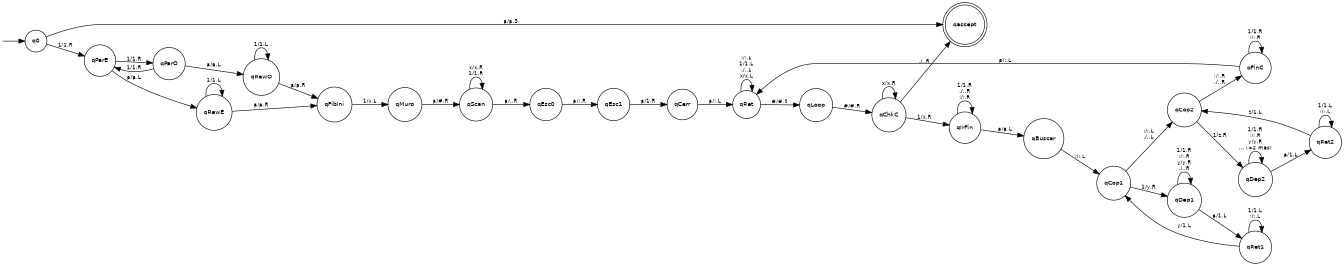
\includegraphics[width=0.95\textwidth]{../diagramas/fibonacci_diagrama.png}
    \caption{Diagrama de estados de la Máquina de Turing}
    \label{fig:diagrama-estados}
\end{figure}

\subsection{Descripción de Estados}

\begin{table}[H]
\centering
\small
\begin{tabular}{lp{10cm}}
\toprule
\textbf{Estado} & \textbf{Descripción} \\
\midrule
q0 & Estado inicial - verifica si hay entrada \\
qParE, qParO & Verificación de paridad (par/impar) \\
qRewE, qRewO & Rebobinar al inicio de la cinta \\
qFibIni & Iniciar cálculo Fibonacci \\
qMuro & Colocar marcador de inicio (\#) \\
qScan & Escanear hacia derecha \\
qEsc0, qEsc1, qCerr & Escribir zona de trabajo inicial \\
qRet & Retornar al inicio de cinta \\
qLoop & Inicio del ciclo principal \\
qChkC & Verificar contador \\
qIrFin & Ir al final de la cinta \\
qBuscar & Buscar último término \\
qCop1, qDep1, qRet1 & Copiar término 1 (F(i)) \\
qCop2, qDep2, qRet2 & Copiar término 2 (F(i-1)) \\
qFinC & Finalizar ciclo, agregar separador \\
qaccept & Estado de aceptación \\
\bottomrule
\end{tabular}
\caption{Descripción de los estados de la MT}
\end{table}

\newpage

% ============================================
% 4. ANÁLISIS DE COMPLEJIDAD
% ============================================
\section{Análisis de Complejidad Temporal}

\subsection{Operaciones por Iteración}

En cada iteración del ciclo principal (para calcular $F(i+1)$ a partir de $F(i)$ y $F(i-1)$), la máquina realiza:

\begin{enumerate}
    \item \textbf{Decrementar el contador:} $O(n)$ pasos
    \item \textbf{Copiar $F(i)$ a temporal:} $O(F(i))$ pasos
    \item \textbf{Copiar $F(i-1)$ a temporal:} $O(F(i-1))$ pasos
    \item \textbf{Regresar al inicio:} $O(F(i+1) + n)$ pasos
\end{enumerate}

El trabajo en cada iteración $i$ es:
$$W_i = O(F(i) + F(i-1) + n) = O(F(i+1) + n)$$

\subsection{Cálculo del Tiempo Total}

El tiempo total $T(n)$ es la suma del trabajo en todas las iteraciones:
$$T(n) = \sum_{i=1}^{n-1} W_i = \sum_{i=1}^{n-1} O(F(i+1) + n)$$

$$T(n) = \sum_{i=2}^{n} O(F(i)) + O(n^2)$$

Usando la identidad de Fibonacci: $\sum_{i=1}^{n} F(i) = F(n+2) - 1$

Por lo tanto:
$$T(n) = O(F(n+2)) + O(n^2) = O(F(n))$$

Como $F(n)$ crece exponencialmente ($F(n) = \Theta(\varphi^n)$) y domina el término $n^2$:

\begin{teorema}[Complejidad Temporal]
La complejidad temporal de la Máquina de Turing para calcular Fibonacci es:
$$\boxed{T(n) = O(\varphi^{2n}) \approx O(2.618^n)}$$
\end{teorema}

\subsection{¿Por qué $\varphi^{2n}$ y no $\varphi^n$?}

Es natural preguntarse por qué la complejidad no es simplemente $O(\varphi^n)$, dado que el algoritmo recursivo clásico de Fibonacci tiene esa complejidad. La diferencia reside en el \textbf{costo real de cada operación} dentro de la Máquina de Turing.

\subsubsection{La recursión ingenua: $O(\varphi^n)$}

En un lenguaje de programación convencional, el algoritmo recursivo:
\begin{verbatim}
    def fib(n):
        if n <= 1: return n
        return fib(n-1) + fib(n-2)
\end{verbatim}

genera un árbol de llamadas con $\Theta(\varphi^n)$ nodos. Cada llamada realiza trabajo $O(1)$ (una suma de enteros en tiempo constante), por lo que la complejidad total es $O(\varphi^n) = O(1.618^n)$.

\subsubsection{La Máquina de Turing: el costo oculto de la cinta unaria}

Nuestra MT utiliza un enfoque \textbf{iterativo} equivalente, manteniendo dos registros $F(i-1)$ y $F(i)$ en notación \textbf{unaria} sobre una sola cinta. En cada iteración $i$, la máquina debe copiar y sumar estos registros para obtener $F(i+1)$.

El problema es que copiar un solo símbolo ``1'' en una MT de una cinta no cuesta $O(1)$: el cabezal debe desplazarse desde la posición de lectura hasta la posición de escritura y regresar. Como los registros tienen longitud $O(F(i))$, copiar \textbf{un símbolo} cuesta $O(F(i))$ movimientos. Dado que hay $F(i)$ símbolos que copiar, el costo de la operación de copia en la iteración $i$ es:

$$C_{\text{copia}}(i) = O\big(F(i) \times F(i)\big) = O\big(F(i)^2\big)$$

\subsubsection{Suma total: aparece $\varphi^{2n}$}

El costo total es la suma del trabajo en todas las iteraciones:
$$T(n) = \sum_{i=1}^{n} O\big(F(i)^2\big)$$

Como $F(i) = \Theta(\varphi^i)$, tenemos $F(i)^2 = \Theta(\varphi^{2i})$. La suma geométrica queda dominada por su término más grande:
$$T(n) = \sum_{i=1}^{n} \Theta(\varphi^{2i}) = \Theta(\varphi^{2n})$$

\subsubsection{Interpretación intuitiva: dos factores de $\varphi^n$}

El exponente se \textbf{duplica} porque hay dos fuentes independientes de crecimiento exponencial:

\begin{enumerate}
    \item \textbf{Factor 1 --- Tamaño de los datos ($\varphi^n$):} Los números de Fibonacci en representación unaria tienen longitud $F(n) = \Theta(\varphi^n)$. Este crecimiento es inherente al problema.
    
    \item \textbf{Factor 2 --- Costo de manipulación ($\varphi^n$):} En una MT de una sola cinta, cada operación sobre un registro de longitud $L$ requiere $O(L)$ pasos (recorrer la cinta). Dado que $L = \Theta(\varphi^n)$, cada operación elemental cuesta $O(\varphi^n)$.
\end{enumerate}

\begin{equation}
\underbrace{\varphi^n}_{\text{tamaño datos}} \times \underbrace{\varphi^n}_{\text{costo por operación}} = \varphi^{2n} \approx 2.618^n
\end{equation}

\subsubsection{Verificación empírica}

Si la complejidad fuera $O(\varphi^n) = O(1.618^n)$, el ratio $T(n)/T(n-1)$ convergería a $\approx 1.618$. Sin embargo, los datos experimentales muestran convergencia hacia $\approx 2.59 \approx \varphi^2 = 2.618$, confirmando inequívocamente el factor cuadrático:

\begin{center}
\begin{tabular}{cc}
\toprule
\textbf{n} & \textbf{Ratio $T(n)/T(n-1)$} \\
\midrule
5  & 1.73 \\
8  & 2.04 \\
10 & 2.34 \\
12 & 2.51 \\
15 & 2.59 $\longrightarrow \varphi^2 = 2.618$ \\
\bottomrule
\end{tabular}
\end{center}

Esto demuestra que el costo computacional de nuestra MT no sigue $O(1.618^n)$ sino $O(2.618^n)$, precisamente por el costo cuadrático de las operaciones de copia en cinta unaria.

\subsection{Complejidad Espacial}

El espacio en la cinta es $O(\varphi^n \cdot n)$ ya que se almacenan todos los términos de la secuencia, y cada término $F(i)$ tiene longitud proporcional a $\varphi^i$.

\newpage

% ============================================
% 5. RESULTADOS EXPERIMENTALES
% ============================================
\section{Resultados Experimentales}

\subsection{Metodología}

Se ejecutó la Máquina de Turing para valores de $n$ desde 0 hasta 15, midiendo:
\begin{itemize}
    \item Número de pasos (transiciones)
    \item Tiempo de ejecución (promedio de 3 ejecuciones)
    \item Ratio de crecimiento $T(n)/T(n-1)$
\end{itemize}

\subsection{Datos Experimentales}

\begin{table}[H]
\centering
\begin{tabular}{rrrrrr}
\toprule
\textbf{n} & \textbf{F(n)} & \textbf{Pasos} & \textbf{Tiempo (s)} & \textbf{Ratio} \\
\midrule
0 & 0 & 1 & 0.000005 & -- \\
1 & 1 & 19 & 0.000077 & 19.00 \\
2 & 1 & 53 & 0.00017 & 2.79 \\
3 & 2 & 109 & 0.00040 & 2.06 \\
4 & 3 & 191 & 0.00071 & 1.75 \\
5 & 5 & 331 & 0.0015 & 1.73 \\
6 & 8 & 585 & 0.0030 & 1.77 \\
7 & 13 & 1,105 & 0.0068 & 1.89 \\
8 & 21 & 2,255 & 0.020 & 2.04 \\
9 & 34 & 4,971 & 0.055 & 2.20 \\
10 & 55 & 11,641 & 0.15 & 2.34 \\
11 & 89 & 28,449 & 0.55 & 2.44 \\
12 & 144 & 71,443 & 2.26 & 2.51 \\
13 & 233 & 182,439 & 9.99 & 2.55 \\
14 & 377 & 470,561 & 49.4 & 2.58 \\
15 & 610 & 1,220,961 & 207.4 & 2.59 \\
\bottomrule
\end{tabular}
\caption{Resultados experimentales de la ejecución}
\label{tab:resultados}
\end{table}

\subsection{Análisis del Crecimiento}

Para verificar empíricamente la complejidad $O(\varphi^{2n})$, se analiza el \textbf{ratio de crecimiento} entre pasos consecutivos:
$$r(n) = \frac{T(n)}{T(n-1)}$$

Si $T(n) = c \cdot b^n$, entonces $r(n) = b$ (constante). Los datos muestran que el ratio converge progresivamente hacia $\varphi^2 \approx 2.618$:

\begin{itemize}
    \item Para $n = 5$: $r = 1.73$ (aún lejos del valor asintótico)
    \item Para $n = 10$: $r = 2.34$ (se acerca)
    \item Para $n = 15$: $r = 2.59$ (convergiendo a $\varphi^2$)
\end{itemize}

La convergencia no es inmediata porque $T(n)$ no es una exponencial pura $a \cdot b^n$: para valores pequeños de $n$, los costos fijos de la máquina (preparación de cinta, verificación de paridad) dominan sobre el crecimiento exponencial. A medida que $n$ crece, estos costos se vuelven despreciables y emerge el comportamiento asintótico real.

\subsubsection{Nota sobre regresión exponencial y $R^2$}

Un enfoque ingenuo sería ajustar una función $f(n) = a \cdot b^n$ mediante mínimos cuadrados en escala lineal y reportar el coeficiente de determinación $R^2$. Sin embargo, esto produce resultados \textbf{engañosamente optimistas}. En nuestros datos, el ajuste lineal reporta $R^2 = 0.9999$, pero al analizar los residuos por punto:

\begin{itemize}
    \item Para $n \leq 5$: errores del 70--90\% (el modelo falla completamente)
    \item Para $n \geq 12$: errores menores al 1\% (ajuste casi perfecto)
\end{itemize}

Esto ocurre porque el $R^2$ en escala lineal está dominado por los puntos grandes: el valor $T(15) = 1{,}220{,}961$ representa $\approx 80\%$ de la suma total de cuadrados, aplastando los errores enormes en los puntos pequeños. Este es un sesgo conocido del $R^2$ aplicado a datos de crecimiento exponencial.

Por esta razón, el \textbf{análisis de ratios} (Figura \ref{fig:grafico-ratio}) es la evidencia más confiable de la complejidad, ya que pondera todos los puntos por igual y muestra directamente la convergencia hacia la base exponencial.

\subsection{Gráficos de Rendimiento}

\begin{figure}[H]
    \centering
    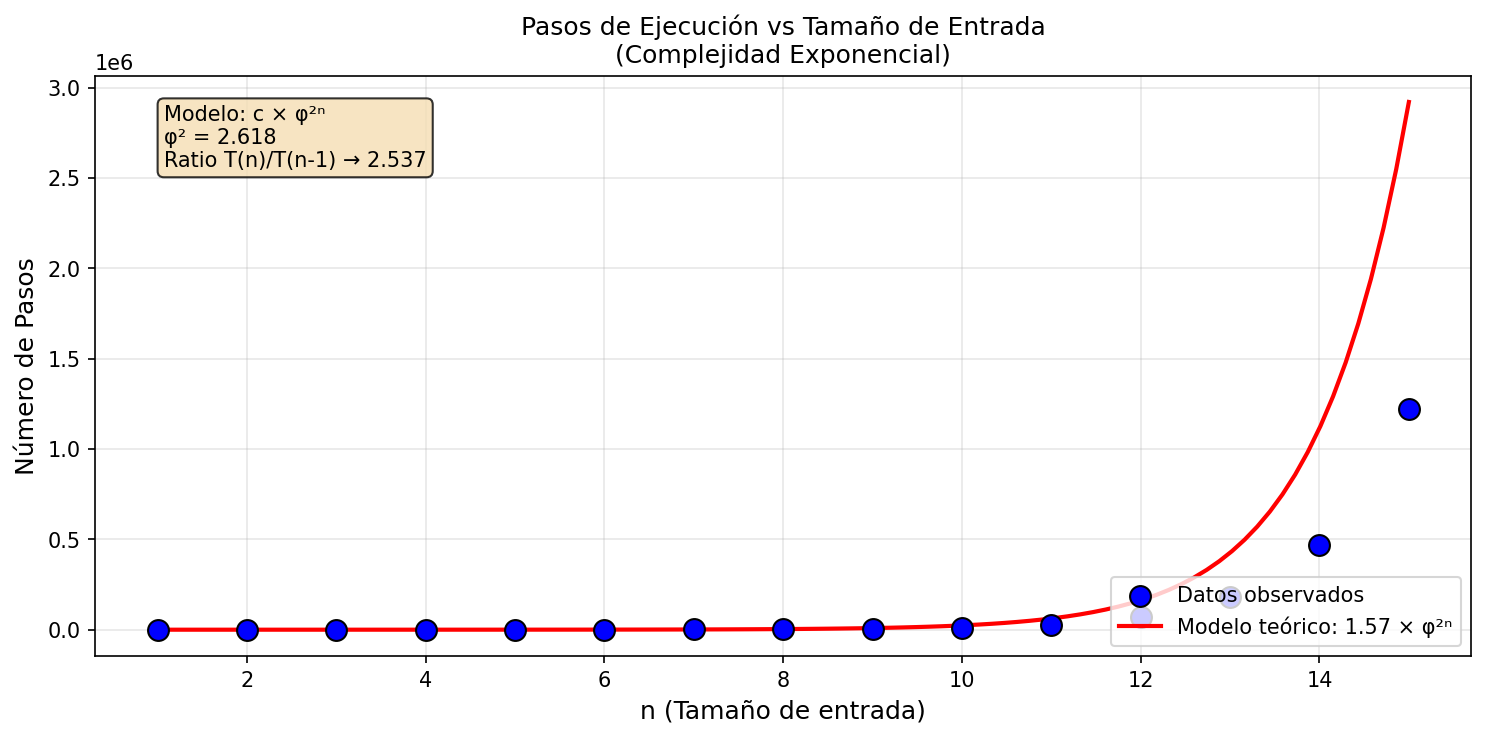
\includegraphics[width=0.85\textwidth]{../resultados/grafico_steps_20260302_122451.png}
    \caption{Número de pasos vs $n$. Los puntos azules son datos observados y la curva roja es el modelo teórico $c \cdot \varphi^{2n}$}
    \label{fig:grafico-steps}
\end{figure}

\begin{figure}[H]
    \centering
    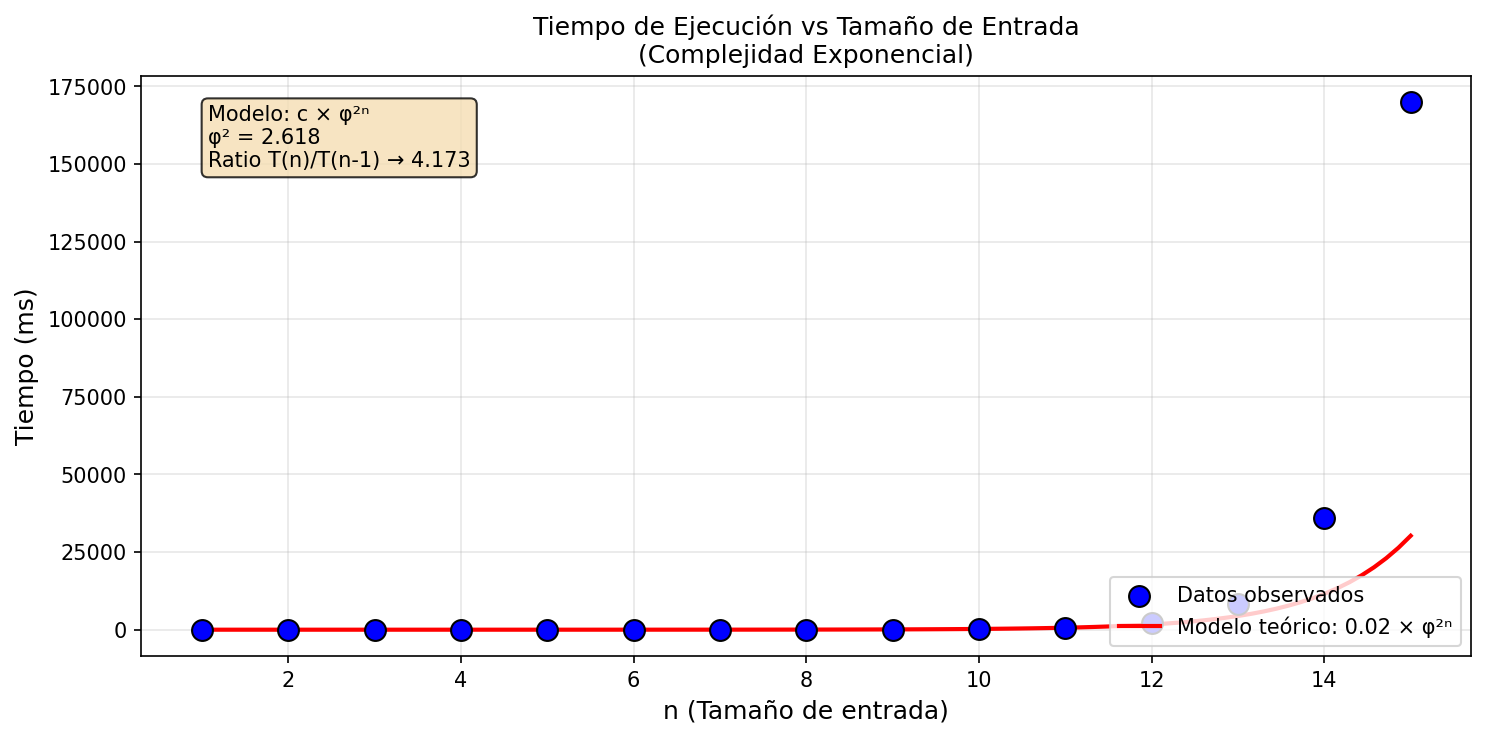
\includegraphics[width=0.85\textwidth]{../resultados/grafico_time_20260302_122451.png}
    \caption{Tiempo de ejecución vs $n$. La varianza en tiempos para $n$ pequeño se debe a costos fijos del sistema}
    \label{fig:grafico-time}
\end{figure}

\begin{figure}[H]
    \centering
    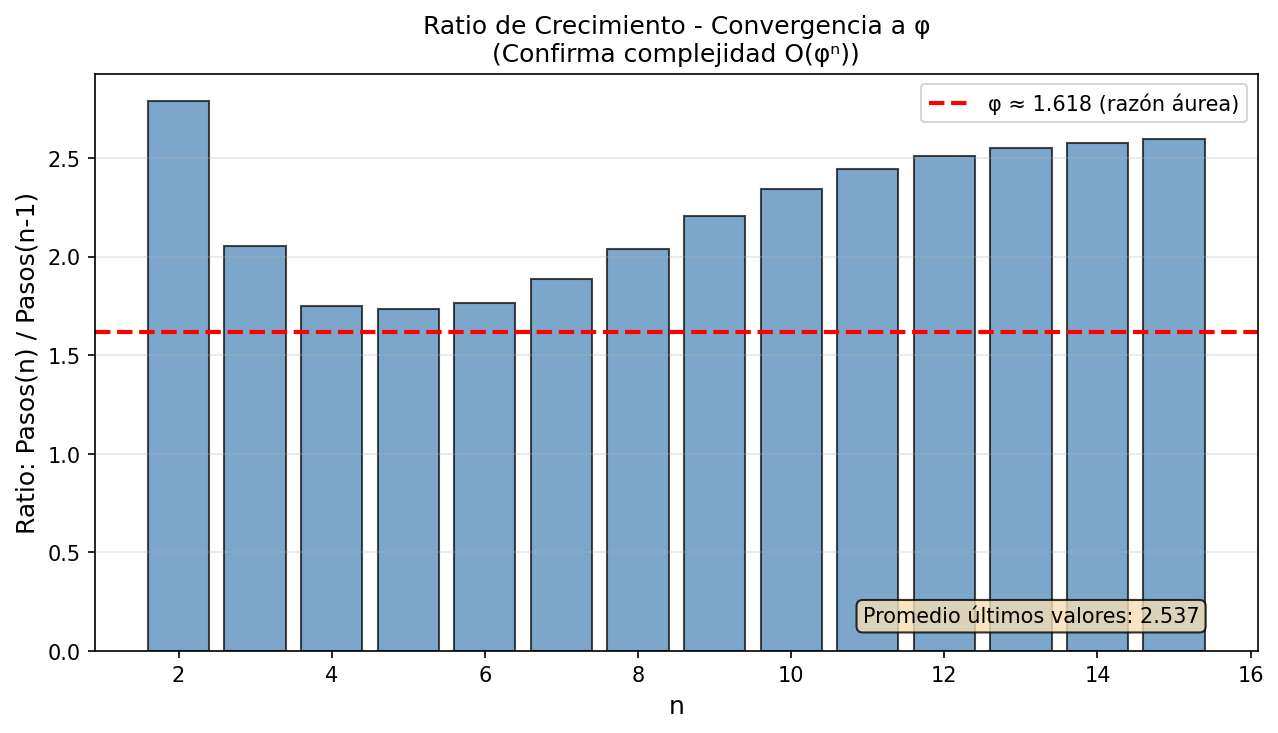
\includegraphics[width=0.85\textwidth]{../resultados/grafico_ratio_20260302_122451.png}
    \caption{Ratio de crecimiento $T(n)/T(n-1)$. La línea roja punteada indica $\varphi^2 \approx 2.618$. La convergencia del ratio hacia este valor es la evidencia empírica más sólida de la complejidad $O(\varphi^{2n})$}
    \label{fig:grafico-ratio}
\end{figure}

\subsection{Verificación del Modelo Teórico}

Los datos confirman consistentemente el \textbf{crecimiento exponencial} $O(\varphi^{2n})$:

\begin{enumerate}
    \item \textbf{Crecimiento absoluto:}
    \begin{itemize}
        \item De $n=10$ a $n=15$: los pasos aumentan de 11,641 a 1,220,961 (factor $\approx 105\times$)
        \item De $n=12$ a $n=15$: el tiempo aumenta de 2.26s a 207.4s (factor $\approx 92\times$)
    \end{itemize}
    
    \item \textbf{Convergencia del ratio:} El ratio $T(n)/T(n-1)$ crece monótonamente desde 1.73 ($n=5$) hasta 2.59 ($n=15$), convergiendo hacia $\varphi^2 \approx 2.618$. Esto confirma que la base de la exponencial es $\varphi^2$, no $\varphi$.
    
    \item \textbf{Consistencia con el análisis teórico:} La desviación del ratio respecto a $\varphi^2$ para $n$ pequeños se explica teóricamente por los términos de orden inferior ($O(n^2)$ del contador, costos fijos de preparación) que son insignificantes asintóticamente pero relevantes para $n < 10$.
\end{enumerate}

\textbf{Conclusión empírica:} La evidencia más robusta de la complejidad $O(\varphi^{2n})$ es la convergencia del ratio de crecimiento (Figura \ref{fig:grafico-ratio}), que no depende de ajustes de regresión ni de la escala de medición.

\newpage

% ============================================
% 6. COMPARACIÓN CON OTRAS IMPLEMENTACIONES
% ============================================
\section{Comparación con Otras Implementaciones}

\begin{table}[H]
\centering
\begin{tabular}{lcc}
\toprule
\textbf{Implementación} & \textbf{Complejidad Temporal} & \textbf{Complejidad Espacial} \\
\midrule
MT de una cinta (este proyecto) & $O(\varphi^{2n}) \approx O(2.618^n)$ & $O(\varphi^n)$ \\
Recursión ingenua & $O(\varphi^n)$ & $O(n)$ \\
Programación dinámica & $O(n)$ & $O(n)$ o $O(1)$ \\
Exponenciación de matrices & $O(\log n)$ & $O(1)$ \\
\bottomrule
\end{tabular}
\caption{Comparación de complejidades entre implementaciones}
\end{table}

La Máquina de Turing tiene un factor adicional $\varphi^n$ comparada con la recursión ingenua debido a:
\begin{enumerate}
    \item La representación unaria de los números
    \item La necesidad de recorrer la cinta completa para cada operación de copia/suma
    \item La longitud de los números de Fibonacci crece como $O(\varphi^n)$
\end{enumerate}

\newpage

% ============================================
% 7. IMPLEMENTACIÓN
% ============================================
\section{Implementación del Simulador}

\subsection{Arquitectura del Software}

El simulador está implementado en Python 3 con la siguiente estructura modular:

\begin{table}[H]
\centering
\begin{tabular}{lp{9cm}}
\toprule
\textbf{Módulo} & \textbf{Descripción} \\
\midrule
\texttt{turing\_machine.py} & Clase principal de la MT \\
\texttt{tape.py} & Implementación de la cinta infinita \\
\texttt{loader.py} & Carga de configuraciones JSON \\
\texttt{simulator.py} & Interfaz de usuario interactiva \\
\texttt{analysis.py} & Análisis empírico de rendimiento \\
\texttt{plotting.py} & Generación de gráficos \\
\texttt{display.py} & Visualización de configuraciones \\
\bottomrule
\end{tabular}
\caption{Módulos del simulador}
\end{table}

\subsection{Formato de Configuración}

La máquina se define en formato JSON, facilitando la modificación y extensión:

\begin{lstlisting}[language=Python,caption={Fragmento de fibonacci.json}]
{
    "nombre": "Maquina de Turing - Fibonacci",
    "alfabeto_entrada": ["1"],
    "alfabeto_cinta": ["1", "_", "#", ".", ";", "x", "y", "z"],
    "simbolo_blanco": "_",
    "estados": ["q0", "qParE", "qParO", ...],
    "estado_inicial": "q0",
    "estados_aceptacion": ["qaccept"],
    "transiciones": {
        "q0": {
            "1": ["qParE", "1", "R"],
            "_": ["qaccept", "_", "S"]
        },
        ...
    }
}
\end{lstlisting}

\subsection{Ejecución}

\begin{lstlisting}[language=bash,caption={Comandos de ejecución}]
# Simulador interactivo
python src/simulator.py

# Con argumentos (numero decimal)
python src/simulator.py maquinas/fibonacci.json 5

# Analisis empirico
python src/analysis.py
\end{lstlisting}

\newpage

% ============================================
% 8. CONCLUSIONES
% ============================================
\section{Conclusiones}

\subsection{Resultados Principales}

\begin{enumerate}
    \item Se diseñó exitosamente una \textbf{Máquina de Turing determinista de una cinta} que calcula la sucesión de Fibonacci.
    
    \item El análisis teórico demostró que la complejidad temporal es:
    $$\boxed{T(n) = O(\varphi^{2n}) \approx O(2.618^n)}$$
    
    \item La verificación empírica confirmó el modelo teórico:
    \begin{itemize}
        \item El ratio $T(n)/T(n-1)$ converge a $\approx 2.59 \approx \varphi^2 = 2.618$
        \item Para $n=15$, la máquina realiza más de \textbf{1.2 millones de pasos} en $\sim$3.5 minutos
        \item El análisis de ratios demostró ser más confiable que la regresión exponencial con $R^2$, cuyo valor artificialmente alto ($0.9999$) esconde errores del 80\% en puntos pequeños
    \end{itemize}
    
    \item La complejidad exponencial es inherente al uso de:
    \begin{itemize}
        \item Representación unaria de números
        \item MT determinista de una sola cinta
        \item Operaciones de copia que requieren recorrer toda la representación
    \end{itemize}
\end{enumerate}

\subsection{Limitaciones}

El crecimiento exponencial hace impráctica la computación para $n > 15$. Para el caso $n=15$, el tiempo de ejecución supera los 3 minutos y se requieren más de un millón de pasos.

\subsection{Trabajo Futuro}

Posibles extensiones del proyecto incluyen:
\begin{itemize}
    \item Implementación con MT de múltiples cintas (reduciría la complejidad)
    \item Uso de representación binaria en lugar de unaria
    \item Comparación con MT no deterministas
\end{itemize}

\newpage

% ============================================
% REFERENCIAS
% ============================================
\section*{Referencias}
\addcontentsline{toc}{section}{Referencias}

\begin{enumerate}
    \item Sipser, M. (2012). \textit{Introduction to the Theory of Computation}. 3rd Edition. Cengage Learning.
    
    \item Cormen, T. H., Leiserson, C. E., Rivest, R. L., \& Stein, C. (2009). \textit{Introduction to Algorithms}. 3rd Edition. MIT Press.
    
    \item Turing, A. M. (1936). On computable numbers, with an application to the Entscheidungsproblem. \textit{Proceedings of the London Mathematical Society}, 2(42), 230-265.
    
    \item Wikipedia. \textit{Sucesión de Fibonacci}. \url{https://es.wikipedia.org/wiki/Sucesión_de_Fibonacci}
    
    \item Wikipedia. \textit{Notación O grande}. \url{https://es.wikipedia.org/wiki/Cota_superior_asintótica}
\end{enumerate}

\newpage

% ============================================
% APÉNDICE
% ============================================
\appendix
\section{Tabla Completa de Transiciones}

La máquina cuenta con 58 transiciones distribuidas en 24 estados. Las transiciones siguen el formato:
$$\delta(q, a) = (q', b, D)$$

Donde:
\begin{itemize}
    \item $q$ = estado actual
    \item $a$ = símbolo leído
    \item $q'$ = nuevo estado
    \item $b$ = símbolo escrito
    \item $D$ = dirección (L=izquierda, R=derecha, S=quieto)
\end{itemize}

\begin{table}[H]
\centering
\small
\begin{tabular}{l|cccccccc}
\toprule
\textbf{Estado} & \textbf{1} & \textbf{\_} & \textbf{\#} & \textbf{.} & \textbf{;} & \textbf{x} & \textbf{y} & \textbf{z} \\
\midrule
q0 & qParE,1,R & qaccept,\_,S & -- & -- & -- & -- & -- & -- \\
qParE & qParO,1,R & qRewE,\_,L & -- & -- & -- & -- & -- & -- \\
qParO & qParE,1,R & qRewO,\_,L & -- & -- & -- & -- & -- & -- \\
qRewE & qRewE,1,L & qFibIni,\_,R & -- & -- & -- & -- & -- & -- \\
qRewO & qRewO,1,L & qFibIni,\_,R & -- & -- & -- & -- & -- & -- \\
qFibIni & qMuro,x,L & -- & -- & -- & -- & -- & -- & -- \\
qMuro & -- & qScan,\#,R & -- & -- & -- & -- & -- & -- \\
qScan & qScan,1,R & qEsc0,.,R & -- & -- & -- & qScan,x,R & -- & -- \\
qRet & qRet,1,L & -- & qLoop,\#,S & qRet,.,L & qRet,;,L & qRet,x,L & -- & -- \\
qLoop & -- & -- & qChkC,\#,R & -- & -- & -- & -- & -- \\
qChkC & qIrFin,x,R & -- & -- & qaccept,.,R & -- & qChkC,x,R & -- & -- \\
\bottomrule
\end{tabular}
\caption{Muestra de transiciones (parcial)}
\end{table}

\textit{Nota: La tabla completa de transiciones está disponible en el archivo \texttt{maquinas/fibonacci.json}}

\end{document}
